% !TeX root = main.tex

\subsection{Simplicial Complexes}\label{sec:complexes}

The notion of a simplicial complex is useful not only as a way to represent our sensor network but also as a convenient way to define homology in the following.
\begin{definition}
   A \textbf{simplicial complex} $K$ is a collection of subsets, called \textbf{simplices}, of a vertex set $V$ such that for all $\sigma\in K$ and $\tau\subset\sigma$ it must follow that $\tau\in K$.
\end{definition}
The \textbf{dimension} of a simplex $\sigma\in K$ is defined as $\dim(\sigma) := |\sigma|-1$ where $|\cdot|$ denotes set cardinality.
The dimension of a simplicial complex $K$ is the maximum dimension of any simplex in $K$.
That is, a graph is a 1-dimensional simplicial complex in which vertices and edges are 0 and 1-dimensional simplices, respectively.

\figblock{%
\begin{figure}[htbp]
\centering
    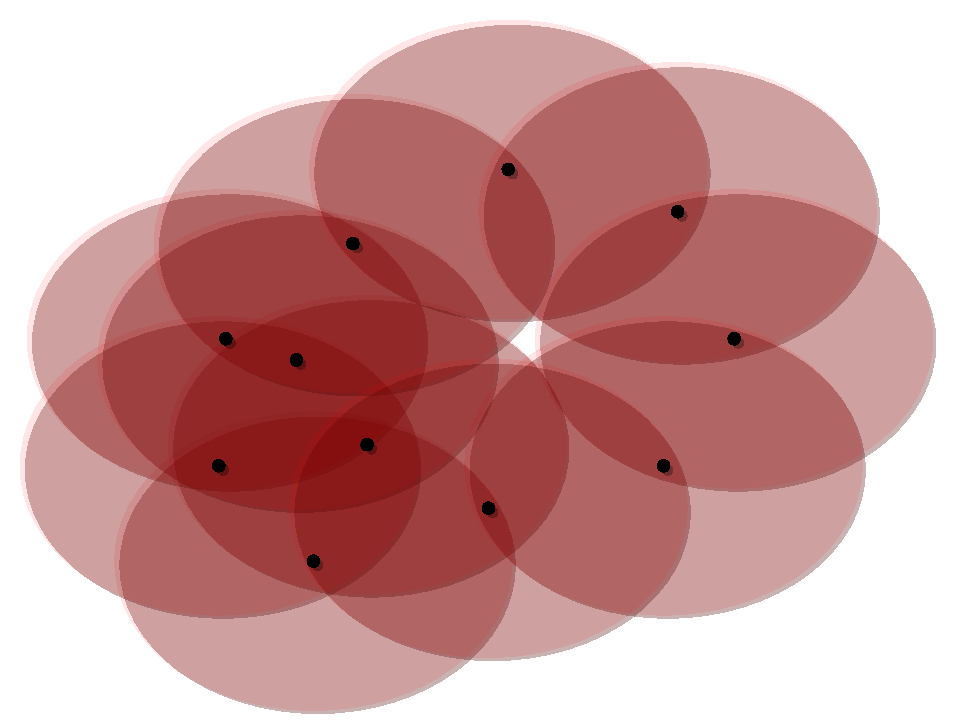
\includegraphics[scale=0.33]{figures/holes_cover.pdf}
    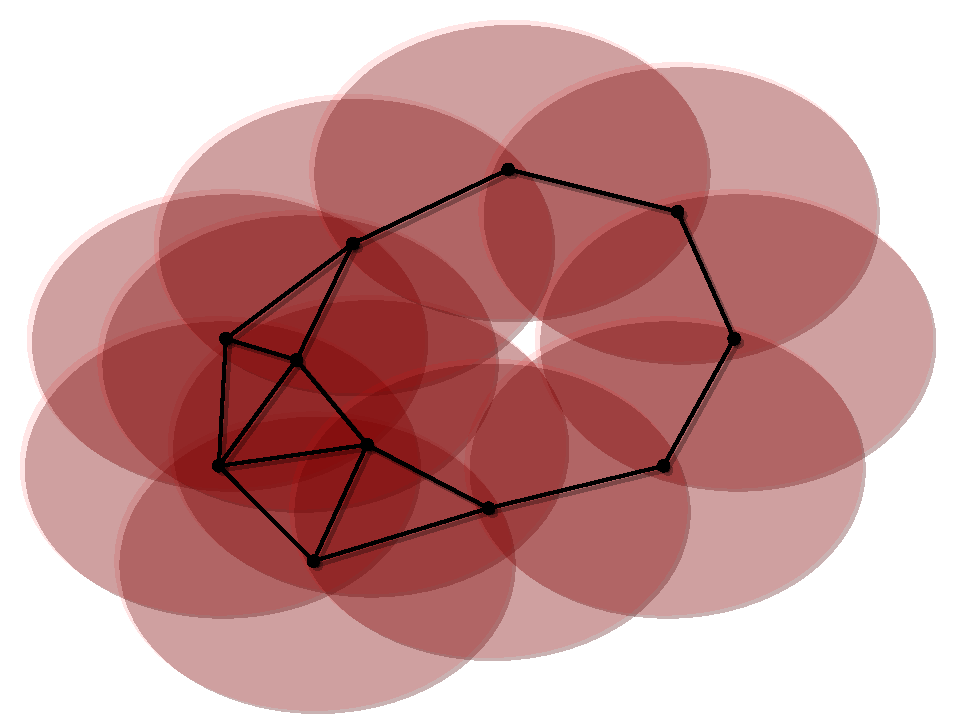
\includegraphics[scale=0.33]{figures/holes_edges.pdf}
    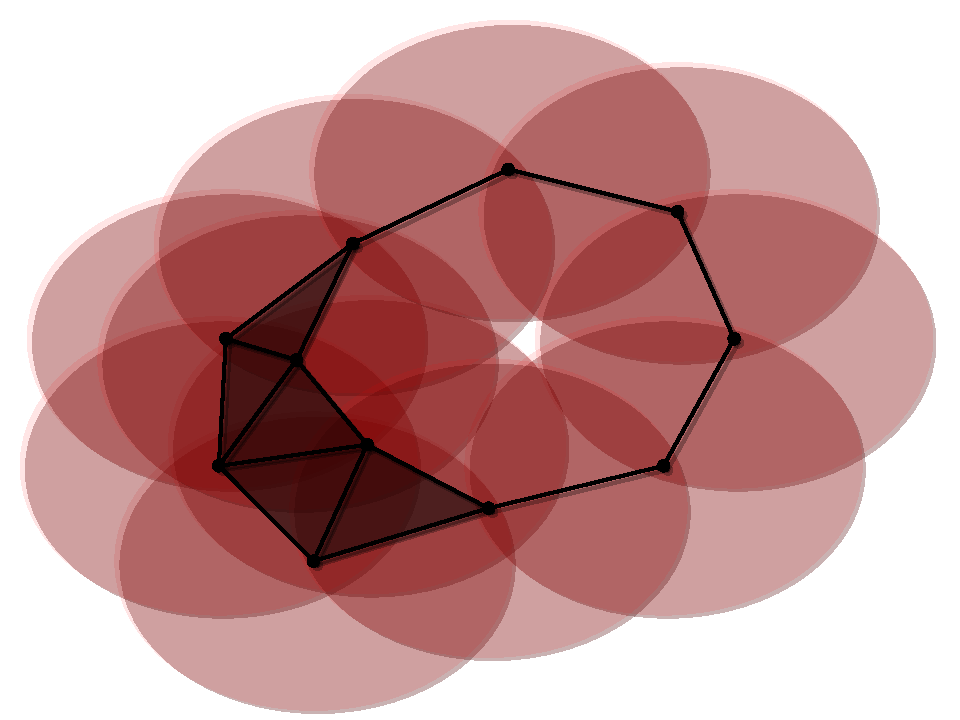
\includegraphics[scale=0.33]{figures/holes_complex.pdf}
     \caption{(Left) The coverage regions of a collection of points $P$ at some scale $\alpha$.
            (Middle) The neighborhood graph with edges for each pair of points within pairwise distance $\alpha$.
            (Right) If we attempt to fill cycles in the graph with triangles identify a cycle that cannot be filled which reflects a gap in coverage}
     \label{fig:holes}
\end{figure}}

It is natural to think of a $k$-dimensional simplicial complex as the generalization of an undirected graph consisting of vertices and edges, collections of at most 2 vertices, to collections of sets of at most $k-1$ vertices.
Just as we have defined a hole in our graph $G$ as a cycle that cannot be filled with triangles, we define a $k$-dimensinal hole in a simplicial complex as a $k$-cycle that cannot be filled with $(k+1)$-simplices.
In the next section we will formally define $k$-cycles and introduce simplicial homology as a tool for identifying when and which cycles cannot be filled.

\paragraph{Coordinate-free Communication}
In a coordinate-free sensor network each sensor, represented by a point in $P$, is capable of detecting nodes which are sufficiently ``close.''
That is, there is some radius of communication $\delta > 0$ such that two nodes $p, q\in P$ such that $\dist(p, q) \leq\delta$ are capable of communication.
Note that, although sensors can communicate within this distance they are not able to measure the distance itself.

With this limited capability we can construct an undirected graph $G=(V, E)$ with vertices $V=P$ and edges $E = \{\{p, q\}\subset P\mid \dist(p,q)\leq\delta\}$.
Let $K$ be a simplicial complex with 0-simplices $\{v\}$ for all $p\in P$, 1-simpices $\{u, v\}\subset P$ for each edge in $E$, and 2-simplices $\{u,v,w\}\subset P$ whenever $\{\{\{u,v\},\{v,w\},\{u,w\}\}\subset E$.
This particular simplicial complex is known as the Vietoris-Rips complex.
It is also an example of a clique complex, where the simplices are the complete subgraphs (or cliques) in a given graph.
\begin{definition}
    The \textbf{(Vietoris-)Rips complex} is defined for a set $P$ at scale $\e > 0$ as
    \[ \rips_\e(P) = \left\{\sigma \subseteq P\mid \forall p,q\in\sigma,\ \dist(p, q)\leq \e\right\}. \]
\end{definition}

\paragraph{Coverage}
% In order to determine coverage we must at least assert that the coverage domain spanned by the points in $P$ does not contain any holes.
% Assuming the coverage radius of our sensors is equal to their communication radius $\delta$ we may define a hole in coverage as a cycle that cannot be ``filled'' with triangles (see Fig.~\ref{fig:holes}).

\figblock{%
\begin{figure}[htbp]
\centering
    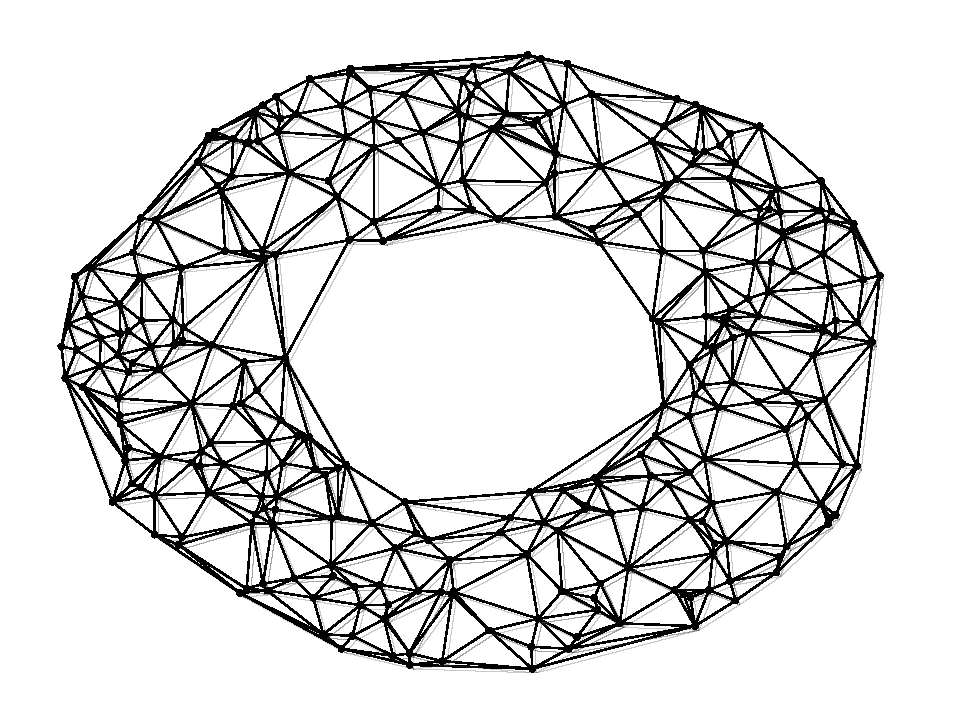
\includegraphics[scale=0.33]{figures/boundary_graph.pdf}
    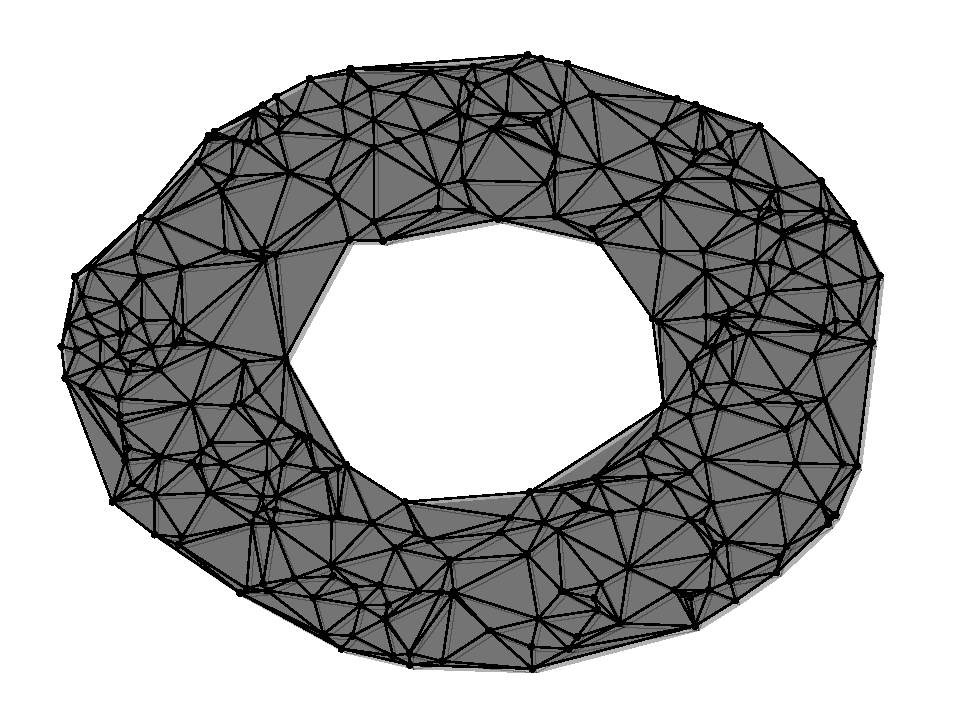
\includegraphics[scale=0.33]{figures/boundary_complex.pdf}
    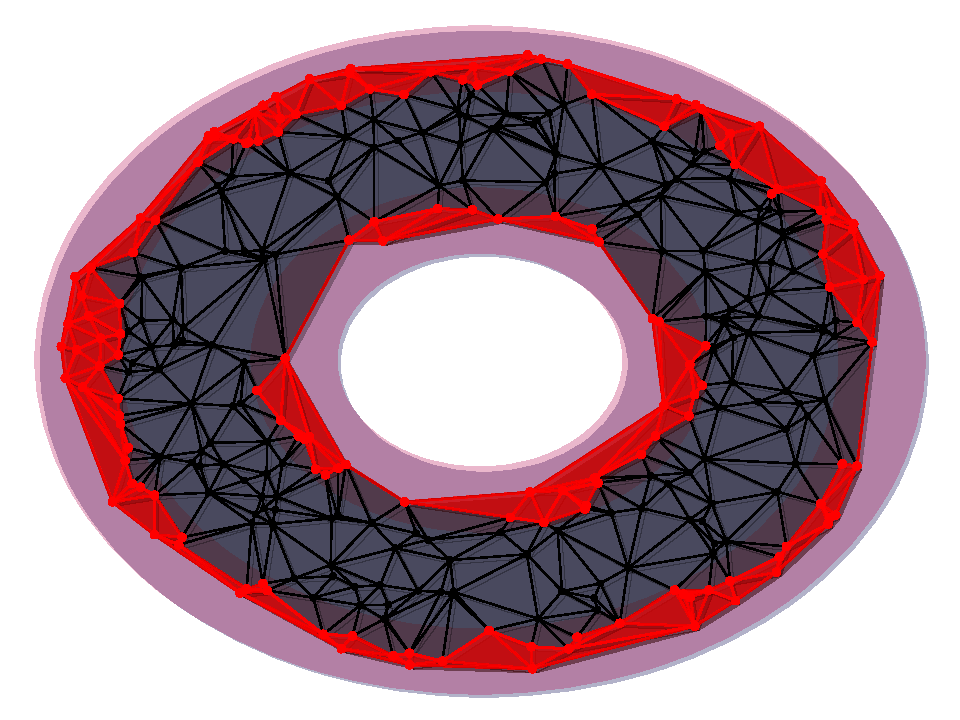
\includegraphics[scale=0.33]{figures/boundary_complex_domain_fence.pdf}
    % 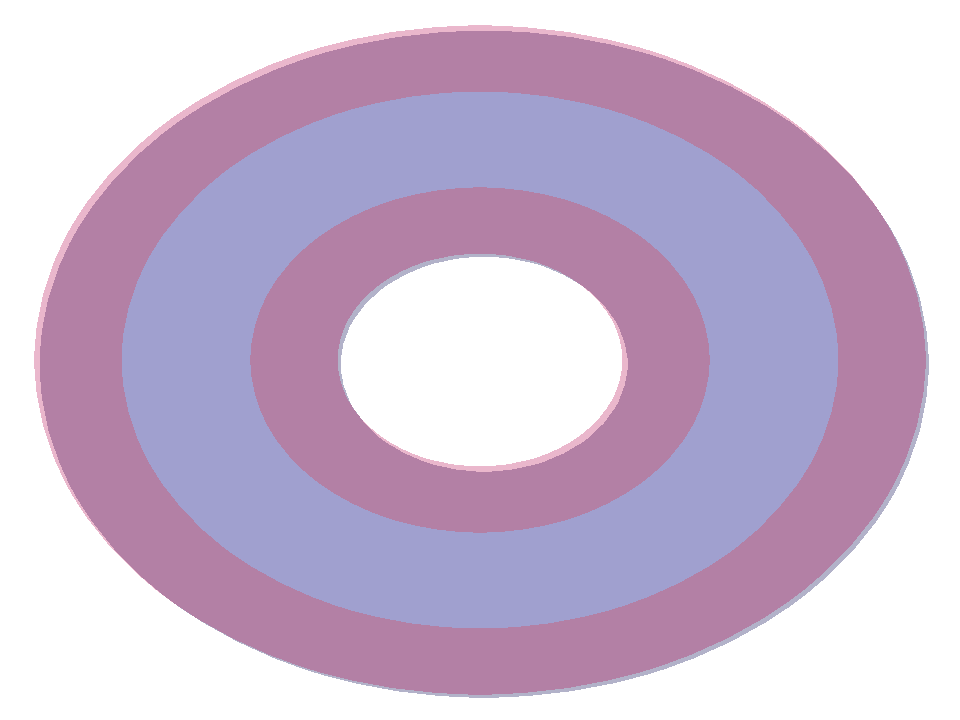
\includegraphics[scale=0.24]{figures/boundary_domain.pdf}
     \caption{(Left) The neighborhood graph of a sensor network with a large ``hole''.
            (Middle) A 2-dimensional simplicial complex with no gaps in coverage, but an unfilled cycle.
            (Right) By allowing nodes to identify the boundary (in red) we can confirm coverage of complex domains.}
     \label{fig:boundary1}
 \end{figure}}

If a sensor network $P$ covers a domain at scale $\e$ the topology of the domain is reflected in $\rips_\e(P)$.
However, as we will see, this does not necessarily give a tight bound on the minimum radius for coverage.
In fact, if the coverage region of of a sensor network at scale $\alpha$ has no gaps, then the minimum coverage radius required is a constant factor smaller than $\alpha$.
This point is made clear by an interleaving of the Rips with another simplicial complex known as the \v Cech complex.

\begin{definition}
    The \textbf{\v Cech complex} of a finite collection of points $P$ at scale $\e > 0$ is defined
    \[ \cech_\e(P) = \left\{\sigma \subseteq P\mid \bigcap_{p\in \sigma}\ball_\e(p)\neq \emptyset \right\}. \]
\end{definition}
The \v Cech complex is a special case of a more general construction known as the \textbf{nerve} $\N(\U)$ of a collection of sets $\U = \{U_i\}_{i\in I}$, where $I$ is any indexing set.
The nerve of $\U$ is defined as the simplicial complex with vertex set $I$ such that $\sigma\subseteq I$ is a simplex if and only if
\[
  \bigcap_{i\in \sigma} U_i\neq \emptyset.
\]
The collection $\U$ is a \textbf{good cover} if for each $\sigma\subset I$ the set $\bigcap_{i\in\sigma} U_i$ is contractible or empty.
The \textbf{Nerve Lemma} states that if $\U$ is a good cover then its nerve $\N(\U)$ is homotopy equivalent to $\bigcup_{i\in I} U_i$.
That is, for a set of nodes $P\subset\D$ such that $\U = \{\ball_\e(p)\mid p\in P\}$ is a good cover the nerve $\N(\U)$ is homotopy equivalent to $P^\e = \bigcup_{p\in P} \ball_\e(p)$.
It follows that the \v Cech complex $\cech_\e(P)$ of $P$ at scale $\e$ is a suitable representation of the coverage region $P^\e$.

\paragraph{Coordinate-free Coverage}
We will assume that the coverage radius of our sensor network is equal to the radius of communication.
In order to construct the \v Cech complex our sensors must be able to measure not only the proximity of neighboring nodes, but the precise distance between them.
Fortunately, the \v Cech and Rips complexes of a finite metric space are closely related by a result that follows from Jung's Theorem~\cite{jung01uber} relating the diameter of a point set $P$ and the radius of the minimum enclosing ball:
\[\cech_{\e/\jungd}(P)\subseteq\rips_\e(P)\subseteq\cech_\e(P)\subseteq\rips_{\jungd\e}(P),\]
where the constant $\jungd = \sqrt{\frac{2d}{d+1}}$ (see~\cite{buchet15efficient}).

Equipped with this interleaving we are now ready to define all conditions necessary for verifying coverage in a coordinate-free sensor network.
Specifically, we will introduce a second radius of communication $\gamma\geq 3\alpha$ that will allow us to lower $\gamma$, which will remain our coverage radius, so that homomorphism on (relative) homology induced by the inclusion of Rips complexes $\rips_\delta(P)\to\rips_\gamma(P)$ reflects that of the \v Cech complex, and therefore the coverage domain.

% In order to \textit{verify} coverage by we need our network to sufficiently sample the extent of our domain.
% Moreover, if there are gaps in coverage, we would like to know if they are due to insufficient sampling or to a gap in the domain itself.
% Let $\B\subset\D$ be the \textbf{boundary} of our domain and let our sensors detect when they are within the communication radius of $\B$.
% Let $Q = \{p\in P\mid \min_{x\in\B}\dist(x, p)\}$ be the set of \textbf{boundary nodes} in $P$.
% The set $Q$ induces a \textbf{subcomplex} $\rips_\alpha(Q)$ of $\rips_\alpha(K)$ restricted to nodes in $Q$.
% % Assuming there are no holes in our network no path from a point in $P\setminus Q$ to a point outside our domain  without crossing a simplex in $K\mid_Q$.
%
% % \textbf{TODO} Section overview.
% % We will show how this construction is used to verify coverage of a specific subset of a bounded domain $\D$ with a tight bound on the coverage radius.
%
% % Note that the communication radius is far from a tight bound on the coverage radius.

% Throughout we have been using the Rips complex as a discrete representation of our coverage domain by assuming the sensor coverage radius is equal to the communication radius.

% section complexes (end)
